%Mark says: This should describe the aims of your research study and why the research problem is important. It should also set the scene for everything that follows.

%Lucie says: 
%*Fact check my %mythology, %science-history and %modern-day-view paragraphs.
%*Fusion
%*Structure
%*Energy transport from core to photosphere
%*Atmosphere (show classic T, rho plot)
%*Magnetic field (permeates entire Sun ands atmosphere)
%   *a couple of statements about internal dynamo
%   *field transported by ("frozen-in") bouyant plasma in the convection zone (flux tubes created by dynamo)
%   *Sunspots to coronal loops
%*Magnetic activity
%   *reconnection
%   *cme
%   *flares   
%*Sunquakes
%*My science question

\section{Introduction}
%Chronological soft intro; use some of the lit review,
%making sure to emphasize the connection to solar flares;Look at early papers predicting sunquakes(Wolff 70s and Kosovichev and Zharkova);the importance of sunquakes
During this age of space-born solar astronomy, understanding the highly dynamic environment of the Sun's atmosphere is a study enriched by a wealth of high detail observations. With each newly launched space instrument the spatial resolution of collected data increases, which coupled with those spacecraft that are tailored to capture light of previously unobserved wavelengths, often leads to new phenomena being observed. Eruptive solar flares fall into this category, in that spacecraft have provided observations that challenge the current theoretical view that the standard eruptive flare model (CSHKP model: \citep{1964NASSP..50..451C, 1966Natur.211..695S, 1974SoPh...34..323H, 1976SoPh...50...85K} puts forward.

Solar flares are one of the most energetic events to occur in the Sun's atmosphere, where by stored magnetic energy is released in the form of heat, mass motions, and accelerated particles. This highly dynamic process produces many measurable emission signatures at wavelengths from $\gamma$-rays to radio waves. Many of these observed signatures agree with the CSHKP model, however, this is not the full picture. The standard flare model has been modified to include new observations many times over the years (e.g., \cite{2011LRSP....8....6S}) and is still unable to describe some observed phenomena. 

Sunquakes are an observable feature during some solar flares that the standard model is unable to explain. It is believed that they are the result of energy and momentum released during the flare impacting the lower solar atmosphere. If a sufficient amount of momentum is imparted on the lowest atmospheric layer, then acoustic waves or 'sunquakes' are produced. The challenges presented in studying this phenomena are mainly associated with the ambiguous nature of the mechanism by which sunquakes are generated. Many ideas for the sunquakes progenitors have been put forward but at this point in time observable signatures do not always show a clear cut evidence aligning with current theories. Therefore this is an exciting time to be investigating the formation mechanisms of sunquakes and could also contribute to our overall understanding of solar flares.      
%%%%%%%%%%%%%%%%%%%%%%%%%%%%%%%%%%%%%%%%%%%%%%%%
%%%%%%%%END OF SOFT INTRO%%%%%%%%%%%%%%%%%%%%%%%
\subsection{Solar Atmosphere}
The solar atmosphere can be described as having four components, the corona, transition region, chromosphere and photosphere, see Figure \ref{solatmpics}.

\begin{figure}[H]%\label{sunquake-cartoon}
  \begin{center}
  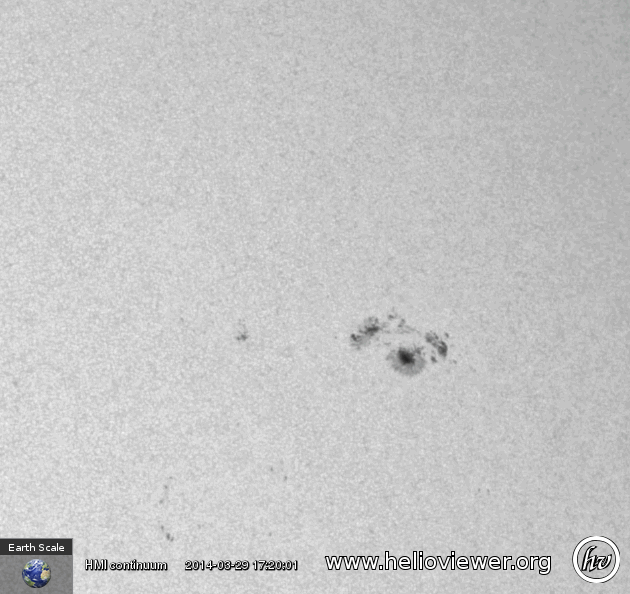
\includegraphics[width=0.20\textwidth]{2014_03_29_17_19_42_HMI_Int}%photsphere
  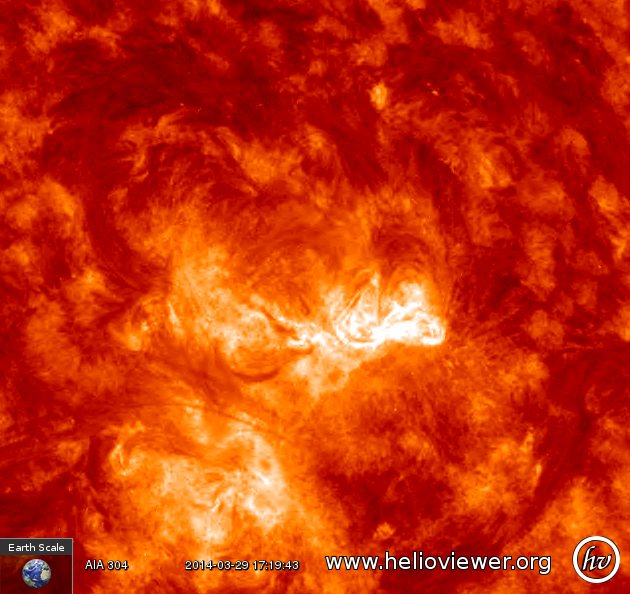
\includegraphics[width=0.20\textwidth]{2014_03_29_17_19_42_AIA_304}%chromosphere
  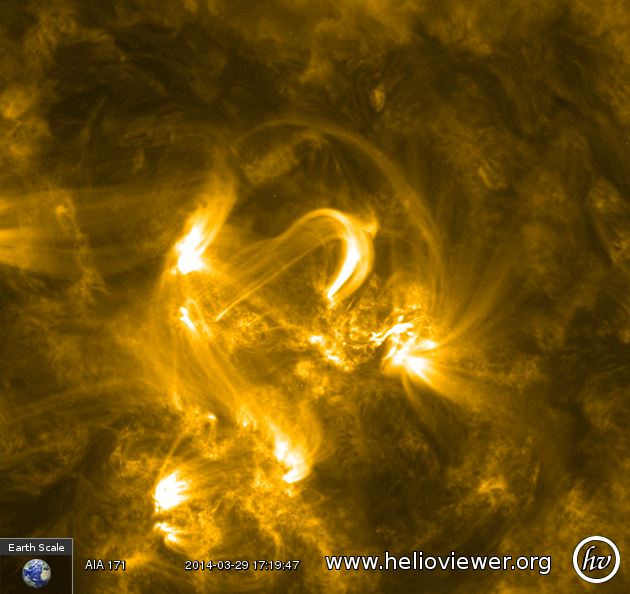
\includegraphics[width=0.20\textwidth]{2014_03_29_17_19_42_AIA_171}%tr
  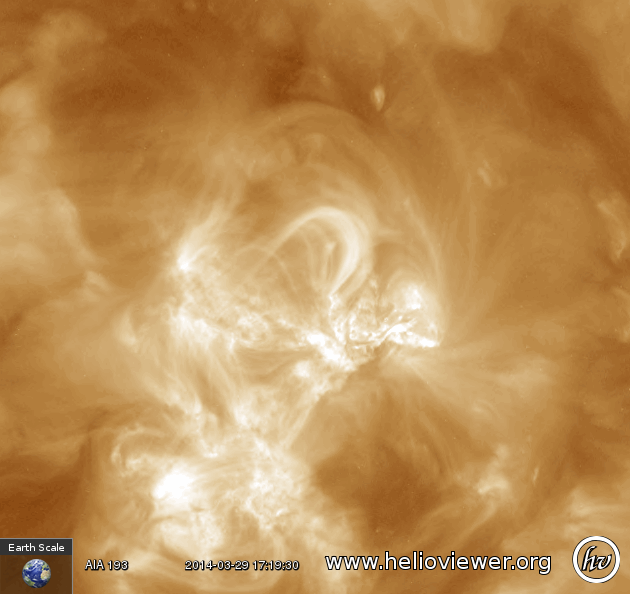
\includegraphics[width=0.20\textwidth]{2014_03_29_17_19_42_AIA_193}%corona
  \caption{ Images taken from the Solar Dynamics Observatory (SDO) instruments, the Helioseismic Magnetic Imager(HMI) and the Atmospheric Imaging Assembly (AIA) displaying the four main components of the solar atmosphere. From left to right layers of the solar atmosphere are increasing in altitude and temperature from the photosphere (SDO/HMI 6173 \AA\ continuum), to the chromosphere (SDO/AIA 304 \AA) through the transition region (SDO/AIA 171 \AA) then up to the corona (SDO/AIA 193 \AA). Images courtesy of \href{www.helioviewer.org}{www.helioviewer.org}}\label{solatmpics}
\end{center}
\end{figure}


For a sunquake to occur, energy released during a solar flare has to traverse these four layers propagating through many pressure scale heights as it does so. Pressure scale height is a measure of the distance over which pressure drops off by a factor of \emph{e}. For example, in the photosphere, $H\sim150$km, whereas in the corona, $H\sim100$Mm. Figure \ref{solatm} shows how the solar atmosphere changes with height, temperature and density, for each of the atmospheric layers. Information in this section is taken from text books: \cite{2003dysu.book.....D, 2004soas.book.....F}


\subsubsection{The Photosphere}
The photosphere is the lowest in altitude of the atmospheric layers, forming a shell around the Sun with a radius somewhere between $\sim10$ - $10^{2}$ km. With an effective temperature of $T\sim5800$K, the photosphere decreases in temperature with radial distance to $\sim4400$K in the temperature minimum region. Emission from this part of the atmosphere is predominantly in the visible range. Contained in the photosphere, are neutral hydrogen atoms, ions and electrons. When a neutral hydrogen atom captures a free electron it forms H$^{-}$ ions, which via absorption of UV and infrared radiation increases the opacity of the region. Even though it is thought that electron capture is a rare occurance, the population of H$^{-}$ ions is large enough to count for the majority of the photospheric opacity. The densest atmospheric layer, plasma pressure in the photosphere is domninant over magnetic pressure such that the plasma-beta, $\beta = p_{gas}/p_{mag} >> 1$. Because of frozen-in theorem (see section \ref{}) photospheric plasma dictates the motions of and to some extent, the morphology of the local magnetic field.

Granules are observed over almost the entire photosphere and are the physical representation of convection currents. Seen as the bright central part of the granule, bouyant, heated plasma rises from a region known as the convective zone, underneath the photosphere. As the material cools, it loses it's bouyancy and falls back toward the interior forming the darker areas surrounding the granule known as intergranular lanes.

Active regions on the photosphere contain sunspots, which are regions of intense magnetic field playing host to footpoints of loops that can extend out into interplanetary space. An active region is formed of at least two sunspots of opposing polarity. 
A sunspot is an approximately circular feature, made up of two main parts, the dark central umbra which is surrounded by the slightly lighter penumbra. The umbra hosts magnetic field lines that are tightly packed and pointing radially away from the Sun, whereas the penumbral magnetic field is more horizontal with respect to the solar surface. With a field strength of $\sim 10^{-1}$ Tesla, sunspots are regions in the photosphere where the magnetic pressure is dominant over plasma pressure, such that $\beta << 1$. Meaning that in these regions convection currents and radiative transfer are inhibited, with the latter being the idea behind a sunspot's dark appearance. \\


\subsubsection{Chromosphere}
The next region of the atmosphere is the chromosphere which is situated above the photosphere. This layer of plasma is a few thousand kilometres (2000 - 3000 km) thick and is optically thin to visible light so is difficult to observe against the brightness of the photosphere. The temperature in this layer increases with height from 4400 K at the temperature minimum region to $\sim10^{5}$K near the transition region. As a result, plasma density descreases and $\beta$ drops, crossing unity near the transition region between the upper-chromosphere and corona. This means that the pressure scale height in this region is changing with altitude as a transition from the plasma to magnetic domain occurs. The chromosphere is observable in the optically thick H$\alpha$ line in a red wavelength due to photoelectric processes. Whereas collisionally produced Ca II H & K and Mg II emission are observable in NUV wavelengths. Sunspots still exert enough influence to control chromospheric plasma and thus are still observable. In this region, dense material suspended in magnetic fields, or filaments, can be observed in absorption, or emission at the limb (prominence). Filaments are thought to be the source of mass for coronal mass ejections (CME) due to their location over active regions and a sudden emptying of material during eruptive flares with a CME. 

\subsubsection{Transition Region}
Up in altitude to the interface between the chromosphere and the corona or transition region. This region is a poorly understood layer of the solar atmosphere. What is known, is that; temperatures climb from $\sim10^{5}$ near the chromsphere to $\sim10^{6}$ K at the corona; this region has variable thickness and maybe even orientation; plasma density falls off sharply. This region can be observed in NUV wavelengths such as Si IV.  

\subsubsection{Corona}
The corona is the outer most layer of the atmosphere extending out into interplanetary space.  With a temperature ranging from $T\sim10^{6}$ - $10^{7}$ K, this the hottest part of the atmosphere. Plasma density in this region is very low, leading to a plasma pressure which is much lower than the magnetic pressure resulting in $\beta << 1$. This means that plasma motions are dominated by magnetic fields leading to magnetic loops that can expand almost unhindered. This region is visible in UV emission by super heated plasma and via white light due to Thompson scattering of photospheric light by free electrons and dust in the coronal magnetic field. 



\begin{figure}[H]
  \begin{center}
    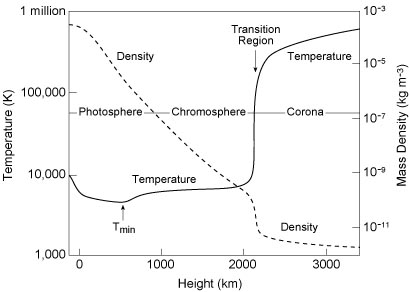
\includegraphics[width=0.6\textwidth]{solar-atm-plot}
\caption{The temperature of the solar atmosphere decreases from values near 6,000 degrees Kelvin at the visible photosphere to a minimum value of roughly 4,400 degrees Kelvin about 500 kilometres higher up. The temperature increases with height, slowly at first, then extremely rapidly in the narrow transition region, less than 100 kilometres thick, between the chromosphere and corona, from about $10^{4}$K to about $10^{6}$K. (Courtesy of Eugene Avrett, Smithsonian Astrophysical Observatory.)}\label{solatm}
  \end{center}
\end{figure}


\subsection{Introduction to Eruptive Solar Flares}

Solar flares are the manifestation of magnetic energy release in the Sun's atmosphere. These events are the most energetic observed solar phenomena, with some of the larger flares releasing up to $10^{37}$ erg of energy. Flares are classified by the the Geostationary Operational Environmental Satellite (GOES) see Table \ref{goes}, in this sytem, the base 10 magnitude of 1 to 8 \AA\ X-ray flux produced by the flare determines it's classification. The GOES system classes flares from X to A-class, in order of high to low flux, so an X-class flare event would be more powerful than an M-class and so on.   \\

\begin{table}[h]
\centering
\begin{tabular}{|c|c|}\label{GOES}
Classification & Peak Flux Range at 1 to 8 \AA\ ($W.m^{-2}$)\\
\hline
X & $10^{-3}$ - $10^{-4}$\\
M & $10^{-4}$ - $10^{-5}$\\
C & $10^{-5}$ - $10^{-6}$\\
B & $10^{-6}$ - $10^{-7}$\\
A & $<10^{-7}$\\
\end{tabular}
\caption{shows the GOES flare classification, which is based on the order of magnitude of hard x-ray flux. X class flares produce a flux of $10^{-3}$ - $10^{-4}$ $W.m^{-2}$ and are the most powerful, whilst a weak A class flare can produce less than $10^{-7}$ $W.m^{-2}$.}\label{goes}
\end{table}

\subsubsection{Flux Emergence}
The exact physical processes governing the trigger mechanism of solar flares are not well understood, however, magnetic reconnection is the commonly accepted theory. So how does magnetic reconnection occur? The process begins with magnetic energy being transported from the solar interior to the atmosphere via flux emergence. At the beginning of a bi-polar active regions life-cycle, a magnetic flux tube emerges from deep in the convective zone. This is due to a high magnetic field strength creating a situation where the plasma density in the flux tube is lower than that of the surrounding plasma. At this point the flux tube becomes bouyant and rises up through the convective zone, emerging at the photosphere. The newly emerged flux rope expands into the atmosphere, driven by a lorentz force exerted by the act of strong electric currents flowing transversally across magnetic field lines. Currents that are aligned to the magnectic field in the flux tube do not generate a lorentz force and thus play no part in the early expansion. Instead, the field-aligned current is fed into the upper portion of the expanded magnetic structure high up in the corona. In the corona, magnetic pressure is much greater than the plasma pressure and as a result this region has low density and high conductivity. If conductivity is high then resitivity is low meaning that dissipation of electric current does not occur, instead the current is stored as an energy, which is released during a solar flare. So as a result of flux emergence, a situation has arisen whereby a magnetic flux loop exists that stretches from the sub-photosphere out into the corona. 

\subsubsection{Magnetic Reconnection}



\subsubsection{2D Flare Model}

\paragraph{Mass Ejection}
\paragraph{Particle Acceleration}
\paragraph{Radiative Energy}
Gamma rays
HXR 
SXR
Radio
UV:
    Hydrogen recombination in the chromosphere?
WLF: 
    How are they formed? Particle bombardment or radiative backwarming, or both?
\paragraph{Shocks and Heating}


The standard 2D flare model is the culmination of research by many authors,\citep{1964NASSP..50..451C, 1966Natur.211..695S, 1974SoPh...34..323H, 1976SoPh...50...85K}, and is still an ongoing area of research that is not entirely understood \citep{2011LRSP....8....6S}. In an active region, a closed magnetic field harbouring a flux rope suddenly opens. As a result, plasma flows along the open field lines from the chromosphere to the corona. This flowing chromospheric material experiences a reduction in plasma pressure which draws together open magnetic field lines of opposing polarity causing reconnection and forming new magnetic loops at lower altitudes. Reconnection causes excess heating at the peaks of newly connected loops which conducts down toward the chromosphere. Also, particles are accelerated by the new magnetic configuration, flowing to the chromosphere. This injection of thermal energy and accelerated particles heats the chromosphere causing HXR footpoints \citep{1995ApJ...455..347A} and UV ribbons \citep{2009A&A...493..241F}. As a result, some chromospheric material evaporates upward into newly created flare loops, whilst some material propagates downward toward the lower chromosphere. The flare loop cools and the process starts again in the next consecutive loop until the unstable magnetic field has relaxed to a state that is closer to it's stable,  potential state.

 In eruptive flares, energy is released every time a new reconnection of a neighbouring loop occurs, this is the reason that flare ribbons appear move away from each other as the flare evolves. \\

White light flares (WLFs) are associated with the most energetic of solar flares. They occur when flare energy is transported deep into the dense lower atmosphere causing an enhancement in optical wavelengths. It is thought this happens due to an energetic particle beam transporting energy to the lower atmosphere where it's energy dissipates into the dense chromospheric or photospheric material. The collisional thick target model by \cite{1971SoPh...18..489B} says that almost all of the flare energy is carried by the particle beam, therefore, energy dissipated in the lower atmosphere represents a large portion of the flare energy budget. White light enhancement from the lower atmosphere can be explained by either Balmer \& Paschen continuum emission from the chromosphere caused by hydrogen recombination, or direct photospheric heating \citep{2007ASPC..368..417D} by radiative backwarming \citep{1989SoPh..124..303M}.


\begin{figure}[H]
  \begin{center}
  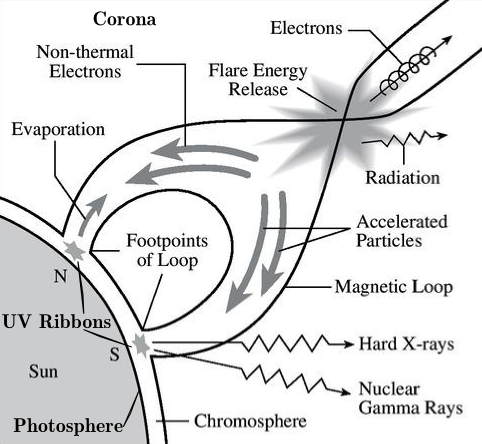
\includegraphics[width=0.40\textwidth]{flare}
  \caption{cartoon of the standard 2D solar flare model. Image courtesy of \href{http://ase.tufts.edu/cosmos/print_images.asp?id=47}{www.tufts.edu}}\label{flare-cartoon}
\end{center}
\end{figure}


%%%%%%%%%%%%%%%%%%%%%%%%%%MHD of solar flares%%%%%%%%%%%%%%%%%%%%%%%%%%%5
\subsection{Solar Magnetohydrodynamics}\label{MHD}
Most structures observed in the solar atmosphere are a direct result of interplay between plasma and the Sun's dynamic magnetic field. Understanding the relationship between a magnetic field and a plasma is important for describing many observed phenomena. Magnetohydrodynamics (MHD) is a method to determine the continuous macroscopic behaviour of plasma in a magnetic field, thus individual particles are not considered \citep{1982soma.book.....P}. A plasma can be treated as a continuous material if distances between particles are much larger than the mean-free path, or larger than the ion gyro-radius. Where $T$ is plasma temperature, $\lambda_{MFP}$ is mean-free path and $n$ is number of particles in the plasma, equation \ref{meanfreepath} describes the mean-free path. 

\begin{equation}\label{meanfreepath}
\lambda_{MFP}\approx300(\frac{T}{10^{6}K})^{2}(\frac{n}{10^{17}m^{-3}})^{-1}m
\end{equation}

Equation \ref{iongyroradius} is the relationship between particle mass $m$, velocity perpendicular to the magnetic field $v_{\bot}$, charge $q$ and magnetic field strength $B$  which governs the circular motion of a charged particle around a uniform magnetic field or the ion gyro radius. 

\begin{equation}\label{iongyroradius}
r_{g}=\frac{mv_{\bot}}{|q|B}
\end{equation}

In the context of the Sun, and the importance of magnetic fields for processes such as solar flares, MHD builds on the following physical assumptions; a magnetic field can manipulate a plasma by exerting a force on it. Leading to the formation of structure or movement via acceleration; a magnetic field can store the energy required for later release as a solar flare; material wrapped in a magnetic field is thermally protected from it's surroundings; a magnetic field can act as a funnel for plasma and fast particles; and finally, a magnetic field can drive instabilities and support waves \citep{2003dysu.book.....D}.

\subsubsection{MHD Equations}\label{MHDeqns}
Magnetic fields are made up of discreet bundles of magnetic flux known as \emph{flux tubes}. A magnetic flux tube can be thought of as cylindrical in geometry and containing magnetic field lines parallel in orientation to the length of the cylinder. The cross-sectional radius of the tube and magnetic field strength are both variant, magnetic flux contained within the tube however, is constant. Where $\vec{B}$ is magnetic field vector and $\vec{dS}$ is a cross-sectional surface element of the tube, flux $F$ follows the relationship.

\begin{equation}\label{fluxtube}       
F = \int_{S} \vec{B}.\vec{dS}
\end{equation}


The basics of MHD are a built from a combination of Maxwell's electromagnetic equations, material equations, Ohm's law and the fluid dynamics relations. Maxwell's equations and Ohm's law describe electromagnetism in terms of magnetic field $\vec{H}$, magnetic induction $\vec{B}$, magnetic permeability of free space $\mu$, electric field $\vec{E}$, electric displacement $\vec{D}$, electrical permittivity of free space $\epsilon$, charge density $\rho_{c}$ and electric current density $\vec{j}$ 


\begin{equation}\label{max1:ampere}
\nabla\times\vec{H}=\vec{j}+\frac{\partial \vec{D}}{\partial t}
\end{equation}


\begin{equation}\label{max2:faraday}
\nabla\times\vec{E}=-\frac{\partial \vec{B}}{\partial t}
\end{equation}


\begin{equation}\label{max3:gauss}
\nabla\cdot\vec{D}=\rho_{c}
\end{equation}


\begin{equation}\label{max4:nomonopole}
\nabla\cdot\vec{B}=0
\end{equation}

with Ohm's law as,

\begin{equation}\label{ohmslaw}
\vec{E}=\frac{\vec{j}}{\sigma}
\end{equation}

where $\sigma$ is electrical conductivity. The fluid dynamics relations are written in terms of density $\rho$, velocity $\vec{v}$, time $t$, pressure $p$, gas constant $\Re$ and temperature $T$. 
%$\frac{d}{dt}=\frac{\partial}{\partial t}+ \vec{v}\cdot\nabla$, sometimes reffered to as the material derivative, is a way of stating the rate of change with respect to time of the  

\begin{equation}\label{motion}
\rho\frac{d\vec{v}}{dt}=-\nabla p
\end{equation}
 
\begin{equation}\label{masscontinuity}
\frac{d\rho}{dt}+\rho\nabla\cdot\vec{v}=0
\end{equation}

\begin{equation}\label{perfectgaslaw}
p=\Re\rho T
\end{equation}

Equation \ref{motion} is the eqn. of motion describing how the forces are exerted on the fluid are equal to the negative gradient of plasma pressure. Equation \ref{masscontinuity} is the eqn. of mass continuity (mass is conserved), whilst equation \ref{perfectgaslaw} is the perfect gas law relating plasma pressure, density and temperature. The fluid dynamics equations are re-written in terms of MHD by building on the following assumptions: Plasma in a magnetic field experiences the Lorentz force $(\vec{j}\times\vec{B})$, such that a plasma volume element $dV$ carrying a current density $\vec{j}$ per unit volume has the force $\vec{j}dV\times\vec{B}$ exerted on it in a perpendicular direction to the magnetic field. In order to cater for the extra force, equation \ref{motion} has the term $\vec{j}\times\vec{B}$ added to the right hand side.   
Ohm's law states that an electric field in the plasma's frame of reference is proportional to the current, however, the total electric field associated with the movement of plasma is $\vec{E}+\vec{v}\times\vec{B}$ ($\vec{E}$ is the electric field acting on the plasma at rest) therefore, equation \ref{ohmslaw} has the term $\vec{v}\times\vec{B}$ added to it's left hand side.The displacement current term $\frac{\partial \vec{D}}{\partial t}$ in equation \ref{max1:ampere} is neglected due to plasma speeds being much slower than the speed of light.

\subsubsection{Induction Equation}\label{inductioneqn}  
Rewriting equations \ref{max1:ampere}, \ref{max2:faraday} and \ref{ohmslaw} using the assumptions from section \ref{MHDeqns}, with $\nabla\cdot\vec{B} = 0$,

\begin{equation}\label{new1}
\vec{j}=\nabla\times\frac{\vec{B}}{\mu}
\end{equation}

\begin{equation}\label{new2}
\frac{\partial \vec{B}}{\partial t} = - \nabla\times\vec{E}
\end{equation}

\begin{equation}\label{new3}
\vec{E}=-\vec{v}\times\vec{B}+\frac{\vec{j}}{\sigma}
\end{equation}

then substituting \ref{new1} solved for $\vec{j}$ into \ref{new2} we have,

\begin{equation}\label{new4} 
\vec{E}=-\vec{v}\times\vec{B}+\nabla\times\frac{\vec{B}}{\eta} 
\end{equation}

where magnetic diffusivity $=\eta =\frac{1}{\mu\sigma}$.

Substituting \ref{new4}, solved for $\vec{E}$, into \ref{new2},

\begin{equation}\label{new5}
\frac{\partial \vec{B}}{\partial t}=-\nabla\times(-\vec{v}\times\vec{B} + \nabla\times\vec{B}\eta)
                                   =\nabla\times(\vec{v}\times\vec{B})-\nabla\eta\times(\nabla\times\vec{B})
\end{equation}

using the vector identity, $\nabla\times(\nabla\times\vec{A})=\nabla(\nabla\cdot\vec{A})-\nabla^{2}\vec{A}$ the last term in equation \ref{new5} becomes $\nabla(\nabla\cdot\vec{B})-\nabla^{2}\vec{B}$, of which the $\nabla\cdot\vec{B}$ term reduces to zero due to equation \ref{max4:nomonopole}, thus we are left with the induction equation \ref{induction} below. 



\begin{equation}\label{induction}
\frac{\partial \vec{B}}{\partial t}=\nabla\times(\vec{v}\times\vec{B})+\eta\nabla^{2}\vec{B}  
\end{equation}

This equation \ref{induction} can be used to determine $\vec{B}$ if $\vec{v}$ is known. The magnetic Reynolds number,

\begin{equation}\label{reynolds}
R_{m} = \frac{l_{0}v_{0}}{\eta} \sim \frac{\nabla\times(\vec{v}\times\vec{B})}{\eta\nabla^{2}\vec{B}}
\end{equation}

is an approximation of the ratio between the first and second terms on the RHS of the induction equation \ref{induction} if $v_0$ and $l_0$ are typical of the velocity and length-scales over which the system is changing. This ratio can be used to diagnose which part of the induction equation is dominating the MHD of the system. For example if $R_m >> 1$ then the $\nabla\times(\vec{v}\times\vec{B})$ term is large and the second term is negligible, so the induction equation becomes,

\begin{equation}\label{r>>1}
\frac{\partial \vec{B}}{\partial t}=\nabla\times(\vec{v}\times\vec{B}),
\end{equation}

thus induction is dominant and Ohm's law \ref{ohmslaw} becomes $\vec{E} +\vec{v}\times\vec{B}$ meaning the total electric field becomes zero.



If $R_m << 1$ then the $\eta\nabla^{2}\vec{B}$ term is large meaning the induction equation becomes,
\begin{equation}\label{r<<1}
\frac{\partial \vec{B}}{\partial t}=\eta\nabla^{2}\vec{B},
\end{equation}

thus diffusion is dominant so the magnetic field $\vec{B}$ will be varying on a length-scale $L_0$, and so will diffuse with velocity \ref{diffvel}, over the time-scale \ref{difftime}.

\begin{equation}\label{diffvel}
v_d=\frac{L_0}{\tau_d} = \frac{\eta}{L_0}
\end{equation}


\begin{equation}\label{difftime}
\tau_d = \frac{L_{0}^{2}}{\eta}
\end{equation}

%check Foukal pg 125 in the pdf
\citep{2003dysu.book.....D}

%puts .tex file here
%\include{example}
\subsubsection{Plasma Beta}
Another way to write the relationship between $\vec{B}$ and $\vec{v}$ is the equation of motion \ref{motion} modified by the Lorentz force.

\begin{equation}\label{motion1}
\rho\frac{d\vec{v}}{dt}=-\nabla p+\vec{j}\times\vec{B}
\end{equation}

The pressure gradient $-\nabla p$ describes the change from high to low plasma pressure. The Lorentz force, $\vec{j}\times\vec{B}$ acts perpendicularly to the magnetic field, therefore accelerated plasma in a direction parallel to the magnetic field is caused by other forces. If equation \ref{new1} is substituted into the Lorentz force,
\begin{equation}\label{lorentzsub1}
\vec{j}\times\vec{B} = (\nabla\times\frac{\vec{B}}{\mu})\times\vec{B}
\end{equation}

then using the triple vector identity, 
\begin{equation}
\frac{1}2{}\nabla(\vec{B}\cdot\vec{B})=\vec{B}\times(\nabla\times\vec{B})+(\vec{B}\cdot\nabla)\vec{B}
\end{equation}

equation \ref{lorentzsub1} becomes,
\begin{equation}
\vec{j}\times\vec{B} = (\vec{B}\cdot\nabla)\frac{\vec{B}}{\mu}-\nabla(\frac{B^2}{2\mu}) 
\end{equation}

therefore \ref{motion1} becomes:

\begin{equation}\label{maghydstat}
\rho\frac{d\vec{v}}{dt}= -\nabla p + (\vec{B}\cdot\nabla)\frac{\vec{B}}{\mu}-\nabla(\frac{B^2}{2\mu}) 
\end{equation}

Because $-\nabla(\frac{B^2}{2\mu}$ is in the same form as $-\nabla p$ it can be said to be the \emph{magnetic pressure}, providing a force pointing from high to low magnetic pressure as $B^2$ changes with position.A measure of dominance of plasma or magnetic pressure in the motion of plasma is known as the plasma beta, 

\begin{equation}\label{beta}
\beta=\frac{p_{plasma}}{p_mag} = \frac{2p_{0}\mu}{B_{0}^2}
\end{equation}

so if $\beta << 1$ then magnetic pressure is dominant and if $\beta >> 1$ then plasma pressure is dominant.

Another useful relationship to use is pressure scale height, where $g$ is acceleration due to gravity and $T_0$ is uniform temperature, pressure scale height, $H=\frac{P_0}{\rho_{0}g} = \frac{\Re T_{0}}{g}$. When combined with pressure, $p$ for a magneto static plasma with uniform temperature, $p=p_{0}\exp^{\frac{-z}{H}}$, where $z$ is altitude, we have a measure of the height, $H$, over which the pressure of a plasma fall off by a factor of $\exp$. 

 %\subsection{Magnetohydrodynamics (MHD)} 



%%%%%%%%%%%%%%%%%%%%%%%%%%%%%%%%%%%%%%%%%%%%%%%%%%%55
\subsection{Sunquakes}
A sunquake occurs when acoustic waves propagate into sub-surface layers of the Sun 
and are then observed on the solar surface as a sunquake (see Figure \ref{sunquake-cartoon}a). As acoustic wave-fronts travel into the interior they encounter layers of increasing density causing refraction back toward the solar surface (see Figure \ref{sunquake-cartoon}b). At which point, waves can be observed as circular formations in the surface plasma, expanding outward from a point of origin (see Figure \ref{mdiquake96}).


\begin{figure}[hb]%\label{sunquake-cartoon}
  \begin{center}
  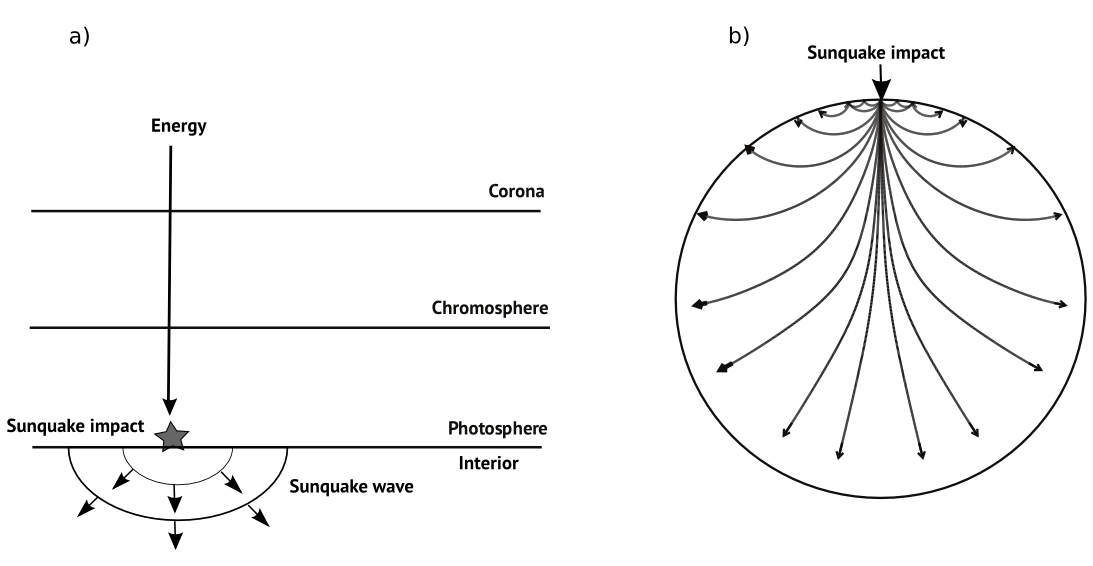
\includegraphics[width=0.99\textwidth]{sunquake-cartoon}
  \caption{Sunquake cartoon: a) Shows a basic picture of sunquake production. Energy moves down through the solar atmosphere impacting the photosphere and generating a sunquake. b) Shows acoustic wave-fronts propagating into the interior of the Sun. Wave-fronts refract back toward the surface as they encounter increasingly dense sub-surface layers. Waves reaching the surface disturb material in a pattern resembling ripples in a pond. Courtesy of \cite{2014arXiv1402.1249K}}\label{sunquake-cartoon}
\end{center}
\end{figure}

\subsubsection{Sunquake Observations}
The idea that solar flares can cause acoustic waves inside the Sun was originally put forward by \citep{1972ApJ...176..833W}. Wolff made the connection that a large solar flare releasing enough energy to heat the photosphere, would generate expansion of photospheric material, which could lead to an impulsive stimulation of oscillations in the Sun's interior. Wolff also commented that it would be difficult to observe interior oscillations with current (in the 1970s) solar velocity measurement techniques.

A little over twenty years later and Wolff's idea was built upon by \cite{1995ESASP.376b.341K}, who showed theoretically that acoustic waves in the solar interior could be generated by a large solar flare, and that they may be detectable. A year later and the first detection of a sunquake was made by \cite{1998Natur.393..317K} during an X class solar flare on July the 9th 1996. Their observational data came from the Solar and Heliospheric Observatory (SOHO) via the Michelson Doppler Imager (MDI) which images the movement of photospheric material by analysing shifts in wavelength of the emitted light. They observed a prominent impulsive downward signature in the Dopplergrams directly over a compact point source which subsequently emanates a set of concentric acoustic waves (see Figure \ref{mdiquake96}). The timing of maximum downward velocity of material derived from the Dopplergrams was out of sync with peak hard x-ray measurements by around a minute. This time delay, coupled with white-light enhancement in the lower atmosphere led to the conclusion that during the flare, accelerated energetic particles heat the cool dense chromosphere causing a shock front which travels downward, depositing energy in lower atmospheric layers, generating a sunquake.

\begin{figure}[hb]
  \begin{center}
  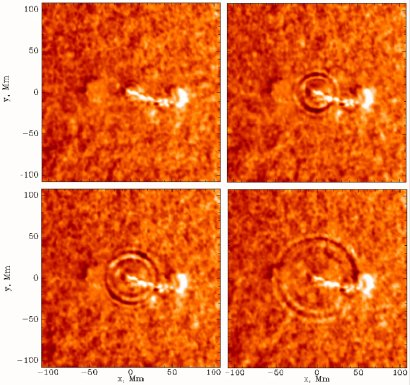
\includegraphics[width=0.80\textwidth]{soho-mdi-quake-96}
\caption{\cite{1998Natur.393..317K} produced SOHO MDI Dopplergrams from the 1996 July 9th, X class solar flare showing the sunquake expanding outward from it's seismic epicentre to a radial distance of $1.2\times10^{8}$ metres. Wave-fronts accelerate from a velocity of 30km/s to 100km/s}\label{mdiquake96}
\end{center}
\end{figure}


The first sunquake observation opened up a whole new area of solar physics, leading to subsequent detections associated other flares. The majority of observations show that sunquakes are often the product of highly impulsive flares, with the acoustic source aligning spatially with white light enhancement in the lower solar atmosphere and hard x-ray emission in the upper-atmosphere \citep{2005ApJ...630.1168D, 2007ApJ...664..573Z}. \cite{2005ApJ...630.1168D} went on to calculate the energy needed to stimulate the propagation of an acoustic wave in the sub-photosphere, finding that only $\sim10^{-3}$ of the energy released by a flare is enough to generate a sunquake. This was an important calculation because it forced the solar community to consider that it might be possible for low energy flares to produce sunquakes, leading to subsequent work by \cite{2008SoPh..251..613M} looking at seismicity of M-class flares.

A paper by \cite{2000ApJ...531L..75H} put forward for the first time, that sunquake production may depend on the changing configuration of the local magnetic field. This idea was further reinforced by \cite{2001ApJ...550L.105K} reporting observations of impulsive changes in magnetic field strength at the photosphere during a solar flare. These magnetic transients were shown to approximately correlate in time and space with hard x-rays, impulsive increases in plasma velocity and increased emission. This line of study was continued \citep{2009MNRAS.395L..39M}, investigating the magnetic field variation of the photosphere in many flares. The study found that some flares with seismicity do not have a spatial and temporal correlation between sunquakes and magnetic transients. Some flares have magnetic transients and no seismicity, and some flares have a good co-spatial alignment of acoustic activity and magnetic variability. It was noted that the impulsiveness of the magnetic field variation could be important as to whether a sunquake is generated.

Some of the most intriguing of sunquake observations are those that do not abide by the usual set of observable features, in that they are not necessarily associated with hard x-rays and excess white-light emission. For example, a statistical survey carried out by \cite{2012SoPh..277..317P}, highlighted a flare containing three footpoints with a seismic source that was co-temporal but not co-spatial with it's closest HXR footpoint; and another source which was co-spatial and co-temporal with its nearest HXR footpoint. This showed that a sunquake does not necessarily correlate with locations of peak emission. Another example by \cite{2011ApJ...741L..35Z} reports an observation of two seismic sources associated with footpoints of an erupting flux rope. During the eruption, the magnetic field above each seismic source undergoes an abrupt permanent reconfiguration. The authors cite the possibility that there exists particle beams low enough in population that HXR emission is undetectable. Further papers investigating the same event \citep{2013SoPh..284..315Z} show that there are downward motions of material above the seismic sources and that energy provided by magnetic transients may not be able to account for the acoustic power generated. These observational oddities prove that mechanisms that generate sunquakes are not well understood and there is much research to be done to classify the different progenitors.

\subsubsection{Sunquake Progenitors}\label{sunprog}
%list and explain current theories of sunquake generation
%making sure to highlight the different observables that can identify each mechanism, eg wlf = evidence of radiative backwarming


The progenitors of sunquakes are still unknown and as a result this is an exciting area of research with discoveries still to be made. The general consensus, in terms of valid mechanisms that could cause this phenomenon is an area of contention, however the following progenitors are thought to be at least partly responsible. \\

\begin{itemize}
\item \textbf{Radiative backwarming} as a mechanism for producing sunquakes, was first put forward by \cite{2005ApJ...630.1168D} to account for a spatial correlation between seismic sources and white light emission from the lower atmosphere. During a solar flare, high energy electrons and impulsively heat the chromosphere and photosphere leading to an enhancement in white light emission \citep{1989SoPh..124..303M}. This WL enhancement can be generated by either; Balmer continuum generated by hydrogen bound-free emission in the upper-chromosphere, which irradiates the photosphere increasing local plasma temperature; $H^{-}$ emission at deeper altitudes, near the temperature minimum region. In both cases, an impulsive increase in radiation pressure and gas pressure exerted on the photosphere could generate acoustic waves which propagate into the sub-photosphere. Therefore a clear radiative energy contribution from Balmer continuum and general white light emission are considered signatures of radiative backwarming. For backwarming to be responisible for the sunquake, a comparable radiative energy budget in a Balmer or white-light signature would be required.\\

\item \textbf{Sudden magnetic field reconfiguration} was first detailed by \cite{2008ASPC..383..221H}. Solar flares are violent physical processes dictated by the interplay between reconnecting magnetic fields and charged solar plasma.
If the magnetic field close to the photosphere relaxes to a more horizontal alignment it can impart a Lorentz force on the local plasma environment, resulting in the production of acoustic waves in the sub-photosphere. The key parameter for this mechanism seems to be that the field has to reconfigure in an sufficiently impulsive manner to generate enough force to induce seismic waves. An observable signature of this progenitor would be impulsive changes in magnetic field strength close to the sunquake. \\

\item \textbf{Shocks} are a mechanism originally proposed in initial work by \cite{1995ESASP.376b.341K} and \cite{1998Natur.393..317K}, whereby a shock wave propagates from the upper-chromosphere down to lower altitudes. During a solar flare, particles and heat are directed down toward the chromosphere, at which point chromospheric material reacts by increasing in temperature. This increased temperature causes explosive ablation of chromospheric material both upward and downward. The downward component develops into a shock front carrying energy to the lower atmosphere, which can go on to impact the photosphere generating acoustic waves. If the shock is dissipated at higher altitudes such as the lower chromosphere, heat generated during the deposition process can irradiate the photosphere with high energy photons, causing radiative backwarming \citep{1989SoPh..124..303M}. Observational signatures of shocks are red or blue shifted wavelengths which can be captured in Dopplergrams or spectroscopic data. \\

\item \textbf{Direct proton collision}, is linked to observations by \cite{2007ApJ...664..573Z} where the sunquake was spatially aligned with $\gamma$-ray emission. $\gamma$-rays during a solar flare are an indicator of energetic protons being accelerated along a newly reconfigured magnetic field. Proton beams carry more momentum than electron beams and are able to penetrate through the solar atmosphere to lower altitudes. If an energetic beam of protons makes it down to the photosphere, it can deposit energy in the form of an impact, which due to conservation of momentum could generate acoustic waves in the sub-photosphere. $\gamma$-ray data is captured by RHESSI. \\

\end{itemize}
%It is also theoretically possible to heat the upper photosphere by resistive dissipation of Alfven waves \citep{1982SoPh...80...99E}


\subsubsection{Local Helioseismology}
%use content from old report...maybe expand a little
Helioseismology is a tool for probing the interior of the Sun. Most techniques in this field of analysis rely on observations of gravity and acoustic waves on the photosphere that are the result of interior excitation. Studying the frequency and modes of these oscillations has revealed much about the internal structure of the Sun. Local helioseismology is a collection of techniques developed for global helioseismology that have been modified for use in studying local regions in higher spatial resolution. The following section provides an introduction to some of these techniques.

\paragraph{Helioseismic Holography}\label{helioholog}
\cite{1999ApJ...513L.143D} pioneered the use of helioseismic holography to produce seismic images of the solar flare of July 1996 reported to have a sunquake by Kosovichev and Zharkova. Time series egression-power maps at 3.5 and 6 mHz were computed with a 2 mHz bandwidth. It was found that the most powerful acoustic power frequency associated with the flare is centred at 3.5 mHz but has a large amount of noise. However, the 6 mHz range has a much lower ambient noise, therefore producing a better rendering of the seismicity of the flare. It is now standard practice to use the 6 mHz range for helioseismic holographic calculations of egression-power. \\
Originally the idea of analysing Doppler images of the solar surface in order to observe acoustic sources was put forward by \cite{1975CRASB.281...93R}. Helioseismic holography was developed further in concept by Lindsey and Braun \citep{1990SoPh..126..101L, 1992ApJ...392..739B, 1997ApJ...485..895L} in an effort to to image the solar interior and far-side of the Sun. This technique involves using a Doppler image of a location on the solar surface as a reference wave-field to enable an estimatation of that wave-field at a location in the solar interior at a time preceding or proceeding the image. This is achieved by calculating the ingression or egression of the wave-field by assuming that it's evolution is a, convergence to, or divergence from, the point of origin of that wave-field. The technique uses Green's function (eqn \ref{green}, where $\vec{r}$ and $t$ are position and time of an observed signal and $\vec{r}'$ and $t$' are the position and time of the signal earlier in time) which assumes that the acoustic wave propagates from a point source, allowing a signal $\psi(\vec{r},t)$ observed on the surface to be devolved backwards in time.

\begin{equation}\label{green}
G_{+}(|\vec{r}-\vec{r}'|,t-t')
\end{equation}

Where $a$ and $b$ constrain the holographic pupil, equation \ref{holog} is then used to devolve the surface signal to calculate the position of subsurface acoustic sources.

\begin{equation}\label{holog}
H_{+}(\vec{r},z,t)= \int dt'  \int_{a<|\vec{r}-\vec{r}'|<b} d^{2}\vec{r}'G_{+}(|\vec{r}-\vec{r}'|,t-t')\psi(\vec{r}',t')
\end{equation}

Equation \ref{eggpower} is then used to calculate the egression power associated with the acoustic sources at a time $t$.

\begin{equation}\label{eggpower}
P(z,\vec{r})=\int dt|H_{+}(\vec{r},z,t)|^{2}dt
\end{equation}

If egression power is required in terms of frequency then equation \ref{eggpower} can be Fourier transformed into frequency space.


\paragraph{Time-Distance}\label{TD}
The first observation of a sunquake \citep{1998Natur.393..317K} used the time-distance technique to track sunquake wavefronts. The paper by \cite{1993Natur.362..430D} explains how to extract time-distance (TD) information from observations of intensity fluctuations on the solar surface. This technique uses travel times of waves between two locations on the solar surface. The method assumes that the travel time of a wave propagating in the interior of the Sun will be modified by any anomalies that it has to travel through, thus the resulting signal will contain the signatures of those irregularities. For instance, if the wave encounters a flow along it's path of travel, it will propagate faster with the flow than against it, affecting travel time.
This technique remaps Dopplergrams into polar coordinates, with the point of origin centred on the area of downflowing material during the flare. This remapped image is then Fourier transformed with respect to azimuthal angle, with the resulting image highlighting circular disturbances as a line of positive slope.
